\documentclass[a4paper,12pt]{report}
\usepackage[tocflat]{tocstyle}
\usepackage[toc,page]{appendix}
\usepackage{appendix}
\usetocstyle{standard}
\usepackage{titlesec}
\usepackage{xcolor}
\usepackage{lipsum}
\usepackage{flafter}
\usepackage{url}
\titleformat{\chapter}
{\normalfont\large\bfseries\centering\uppercase}
    {}{0.5em} {}
\usepackage{tabularx} % extra features for tabular environment
\titleformat{\section}{\normalsize\bfseries\uppercase}{\thesection}{0.5em}{}
\titleformat*{\subsection}{\normalsize\bfseries}
\titlespacing*{\chapter}{0.00in}{-0.5in}{5mm}

\usepackage{tocloft}
\usepackage[english]{babel}
\usepackage{microtype}
\usepackage{amssymb,amsmath,amsthm}
\usepackage{mathptmx}
\usepackage{float}% improve math presentation
\usepackage{graphicx}
\usepackage{dirtytalk}
\usepackage{chemformula}
\usepackage[lmargin=1.5in, rmargin=1.1in, bmargin=1in, tmargin=1in, a4paper]{geometry} % decreases margins
\usepackage{cite} % takes care of citations
\usepackage{gensymb}
\usepackage[final]{hyperref} % adds hyperlinks inside the generated pdf file
\usepackage{etoolbox}
\usepackage{parskip}
\graphicspath{ {./images/} }

\hypersetup{
        colorlinks=false,
        pdfborderstyle={/S/U/W 1},
        pdfborder=0 0 1
}


\pagenumbering{roman}
\linespread{1.5}
\usepackage{eso-pic}
\newcommand\BackgroundPic{%
\put(0,0){%
\parbox[b][\paperheight]{\paperwidth}{%
\vfill
\centering
\includegraphics[width=\paperwidth,height=\paperheight,%
keepaspectratio]{background.png}%
\vfill
}}}
\renewcommand{\contentsname}{}

\begin{document}
\AddToShipoutPicture*{\BackgroundPic}

\title{%
    \textbf{\textcolor{white}{From 'AI' to 'A+'}} \\
    \large \textcolor{white}{Generative Artificial Intelligence in the Classroom}}

\author{\textcolor{white}{Luc Angevare}}

\date{\textcolor{white}{\today}}
\maketitle
\renewcommand{\contentsname}{}
\section*{Table of contents}
\vspace*{-3cm}
\begingroup
\let\clearpage\relax
\tableofcontents
\endgroup

\newpage

\chapter{Introduction} \label{chap:intro}
\newpage

\section{Abstract} \label{sect:abstract}
\hspace{10mm} In an era defined by technological progress and an escalating intricate web of global challenges, education stands as
the key to fostering innovation and addressing the myriad issues facing our world. The question on how machines can be used within civilian life has plagued man since the end of the Second World War. While attempting to formulate an answer to this question, a technological revolution has occurred every decade since. Whether it be the rise of the personal computer, the emergence of the laptop, the later upcoming of smartphones, or the making of various social media. The most recent technological shift is the major switch to generative Artificial Intelligence.


Artificial Intelligence, hereafter AI, had first been introduced as an academic discipline in the Dartmouth Summer Research Project ~\cite{mccarthy55}. The leaders of the summer research project and their students made programs that solved early algebra problems and proved logical theorems. From this point on, the advancements within AI have become exponential, with there being more and more developments per year. Only when the method of deep learning was discovered in 2012, however, did AI become used within many companies and adopted by many people. The amount of publications on AI after the adoption of machine learning has grown by about 50\% ~\cite{unesco2021sciencereport}. Surprising then, should not be that the first Natural Language Processing system that passed the Turing Test – Google’s LaMDA – already passed it about ten years later, in June of 2022. Only two months later, with the release of OpenAI’s ChatGPT, was the Turing Test passed by another Natural Language Processing ‘chatbot’ ~\cite{biever2023chatgpt}. ChatGPT has, since its beta version, gained massive popularity. The milestone of 1 million users was reached within a staggering 5 days, and 100 million was hit within a revolutionary 2 months, according to a study done by ~\cite{hu2023chatgptreuters}. As a comparison, the second fastest platform to hit 100 million users was ByteDance’s TikTok, achieving the milestone within nine months.


However positive these statistics may seem, the unfortunate side is that ChatGPT is certainly not only used for inherently good reasons and outcomes. Wired reports that it only took ‘a few hours’ to jailbreak ChatGPT ~\cite{burgess2023bchatgpthacking}. This had as consequence, meant everybody with bad intentions and an internet connection could easily get information on how to do anything. Examples include stealing a car, making methamphetamines, anything that ChatGPT normally refuses to answer. Besides people with inherently bad intentions, many students have also noticed ChatGPT. Various educational institutions are looking for the solution to the problem that has arisen since the beginning of generative AI. The development of ChatGPT has meant pupils are expected to be less creative, as generative AI may take over a great deal of the creative process. Teachers and schools alike are looking at how to incorporate ChatGPT into their lessons, as combating it is of no more use because of the unmatched speed of its adoption.


As empirical evidence, many teachers have asked me to teach them how to make responsible use of ChatGPT, and how to allow students to utilise ChatGPT, while still allowing them to think for themselves. This study aims to definitively answer whether ChatGPT can be used as a source of facts, while still keeping pupils thinking for themselves, so education and educators can do what they were made to do, provide learning spaces and learning environments for the teaching of pupils. The hope is that the outcome of this research leads to a balanced integration approach, where ChatGPT can be used alongside educational systems.


These quick and big changes to the ecosystem of technology call for agile adjustments within the environment of education and enterprises. However, the structure of specifically school systems, do not allow for rapid revisions within the whole of education. This research aims to solve the question on what the changes within education in specific need to be.

The main research question within this research is as follows: “How can generative AI support teachers in creating effective teaching materials, assessing students, and enhancing student engagement and performance in education?”. To answer this complex and multifaceted question, various subquestions have been formulated:
\newpage

\begin{enumerate}
    \item How does generative AI work?
    \begin{enumerate}
        \item What are the core concepts and techniques behind generative AI?
        \item Which algorithms are commonly used in generative AI systems?
    \end{enumerate}
    \item How is generative AI currently applied in education?
    \begin{enumerate}
        \item What are examples of existing applications of generative AI in education?
    \end{enumerate}
    \item How can generative AI support teachers in creating effective teaching materials?
    \item How can generative AI assist teachers in assessing students?
    \begin{enumerate}
        \item How can generative AI systems be used for automatic grading of assignments and tests?
    \end{enumerate}
    \item How can generative AI improve student performance?
    \begin{enumerate}
        \item What evidence is there to demonstrate that generative AI can actually enhance student performance?
    \end{enumerate}
    \item What are the ethical and privacy considerations when using generative AI in education?
    \begin{enumerate}
        \item What concerns and challenges arise when implementing generative AI in educational institutions?
    \end{enumerate}
\end{enumerate}

\newpage
\section{Hypothesis} \label{sect:hypothesis}
\hspace{10mm} The integration of generative Artificial Intelligence (AI) into educational settings presents a paradigm shift with the potential to revolutionise teaching methodologies and student engagement. Specifically, this research proposes that the incorporation of generative AI, exemplified by platforms such as ChatGPT, can significantly enhance the effectiveness of teaching practices in terms of resource creation, assessment processes, and overall student performance.

Our hypothesis is grounded in the belief that responsible and ethical utilisation of generative AI tools can empower educators by providing innovative solutions for the development of teaching materials. By leveraging the capabilities of generative AI, teachers can streamline the content creation process, ensuring materials are dynamic, relevant, and tailored to the diverse needs of students.

Furthermore, the research suggests that generative AI can streamline assessment procedures, offering efficient and personalised evaluation methods. Automated grading and assessment tools powered by generative AI can assist teachers in providing timely and constructive feedback, allowing for a more nuanced understanding of individual student needs and progress.

Beyond resource creation and assessment, it is anticipated that the integration of generative AI can enhance student engagement and performance. The interactive and responsive nature of generative AI platforms, such as ChatGPT, can create dynamic learning environments, catering to various learning styles and fostering a more interactive educational experience.

However, this study acknowledges the necessity of a balanced integration approach that considers ethical, privacy, and pedagogical concerns. The hypothesis recognizes the importance of preserving critical thinking skills and creativity in students while harnessing the benefits of generative AI. Striking this balance will be crucial in ensuring that the integration of generative AI into educational systems is not only effective but also aligns with the overarching goals of education.

To substantiate this hypothesis, our research will delve into various aspects, including understanding how generative AI works, exploring core concepts and techniques, examining commonly used algorithms, and investigating existing applications of generative AI in education. Additionally, in this research it will be assessed the potential of generative AI in creating effective teaching materials, assisting in student assessments, and improving overall student performance. Ethical and privacy considerations, as well as concerns and challenges related to implementation in educational institutions, will be thoroughly examined to provide a comprehensive understanding of the implications of generative AI in education.

In summary, the study hypothesises that a thoughtfully integrated generative AI can be a transformative force in education, empowering educators and enhancing the learning experience for students. Through rigorous exploration and analysis, this research aims to contribute valuable insights to the ongoing discourse on the role of generative AI in shaping the future of education.

\chapter{Theoretical Framework} \label{chap:theoretical}
\newpage
\section{What is Artificial Intelligence?} \label{sect:AI}
\hspace{10mm} Artificial Intelligence, a term of which the definition was once a matter of debate, has now become one that is a buzzword for a great amount of programs and algorithms. In this research paper, the aim is to utilise the definition written by Sir Alan Turing, within the seminal paper Computing Machinery and Intelligence, released by MIND in October of 1950. Within this paper, Alan Turing wrote and released the well-known Turing test. This research aims itself toward generative artificial intelligence, in which case the Turing test is the only definition this research may need.

Within the Turing test, the question is proposed whether the average person is able to differentiate between the products made by a human and a machine, if the person is unable to distinguish between these, or has the same ratio as random chance, the machine may be called Artificial Intelligence. If they are unable, it is just a machine. Instead of determining whether the machine is artificially intelligent by its code or by the way it produces an output, it is determined by whether the output is humanly understandable and in a way indistinguishable from human intelligence. A good example of a machine having passed the Turing test, and one of the first ones to have publicly done so, is the beta version of ChatGPT.

The question that remains to be answered and defined, is no longer what artificial intelligence is, rather, what generative artificial intelligence - hereafter generative AI - is. Leading companies within graphics and graphical systems such as Nvidia define generative AI as “being able to generate new content based on a variety of inputs”. For this research paper, the definition of Nvidia will be utilised, with a number of changes. The definition within this research paper will be “Artificial Intelligence that has the capability of creating new content based on an input”. With these changes, various programs such as Dall-E or ChatGPT are also included within the scope of this research paper, as the provided examples are able to generate content by only one type of input, textual.

\newpage
\section{How does generative AI work?} \label{sect:work}

\hspace{10mm} Generative Artificial Intelligence (in the tech world better known as General Adverserial Networks (GANs)) are in very many ways alike with examples in the real world, as is the case with most complex technological systems. Generative AI has been modelled after the human brains, with exactly how human neurons fire inline. Generative AI is based on a technique that has been around since 1795, introduced by Gauss to predict planetary movement. Generative AI usually uses a complex Artificial Neural Network architecture, a computational structure inspired by the neural connections in the human brain. In the basis, neural networks operate based off of layers of nodes, these are all interconnected and intertwined by connections known as edges. Each node represents a number, usually between 0 and 1. The number is weighted by training the model, in which it is tested. Here it compares its predictions with the actual outcomes of the training data. This is done using a process called backpropagation, where the network iteratively refines its weights to minimise the error. The layers are usually divided into three: The input, hidden and output layers (see Appendix A \ref{app:a}).

\begin{itemize}
    \item{The input layer, the first layer within a neural network, is responsible for receiving external information, and changing this to individual numbers per node. For example, imagine a neural network with the task of recognizing text within an image; this layer would be responsible for representing the image in numbers. The numerical value of the colour of an image in grayscale, for example.\\
    If the example would be more concrete, visualise a grayscale image of the number 7. This image would have a resolution of 128 pixels by 128 pixels. The input layer then, would have (\(128\times128 =)\) \hspace{.25mm} \(16,384\), \(2^{14}\) nodes. Each pixel has a value between 0 and 255, the value of 255 represents a black colour of the pixel; the number 0 represents white. Divide this value by 255 (the maximum value) and one has achieved the value of each node. This is the image, represented in numerical values. This completes the function of the input layer.}
    \item{The hidden layers process the information from the input layer. Each node in a hidden layer performs a weighted sum of the input values, followed by the application of an activation function. This allows the network to capture complex relationships within the data. This layer is the most indeterminate layer, as everything in this layer is hidden and all processes are determined automatically, adjusted by the training data and the process of backpropagation. This is the layer that does the most, and this layer is the layer that may actually be called 'artificially intelligent'.\\
    Continuing the previously used example, a node of the hidden layer might detect edges in different orientations, each weight determines which features of the numerical input data it is more or less sensitive to. By training and becoming more accurate, the hidden layer starts to identify patterns like edges, curves, or combinations of these in the input data, however, no person, not even the programmer(s) of the neural network, know which features these are. Therefore, the neural network may contain errors or biases by the training data that people may only notice after it has been published. Such was the case with a Twitter bot published by Microsoft, which became racist and misogynistic because of biases within its training data ~\cite{nazibot16}. To provide an example:\\
    \say{[...] bush did 9/11 and Hitler would have done a better job than the monkey we have now. donald trump is the only hope we've got.} — TayTweets (@TayandYou) March 24, 2016
    }
    \item{Finally, the output layer represents the outcome of the decisions made by the hidden layer. It produces the final results of the neural network's computation. The processed information is processed and represented in the desired format. Usually, the node that is activated the highest indicates the neural network's prediction.\\
    To finish the example, the hidden layer may lead to a total of 10 output nodes, each representing a number between 0 and 9. The hidden layer has decided the probability of the image representing each node, and the probability of the number 7 is the highest.}
\end{itemize}

The provided example is one of a common recurring program, named an optical character recognition algorithm. Making a program that uses a rolling window system, taking an image of \(128\times128\) and recognizing character by character. Change the output node from only 10 nodes to 256 (\(2^8\)), making up the most common text encoding UTF-8), the neural network will be able to recognize all characters defined by the Unicode Standard, and will be able to recognize a larger text with complex characters. The example shows the many and multifaceted uses of a simple neural network.

To demonstrate exactly how the average Artificial Neural Network works operates, another example is provided. Presented is a robot pupil of a private school. The robot is in every way the same as any human of adolescent age, except that it has built-in knobs you can turn to change its brain. The robot pupil studies for a test it receives every week, where it must differentiate between images of a bee and images of a dog. Within the school and guiding the pupil, there is a robot teacher. Every day, the teacher only shows the pupil images of bees and dogs; the pupil then makes a test, which is corrected by the teacher who has the answer key. The test consists of only never before seen images of bees and dogs, and the pupil must fill in whether it predicts the image to be of either. When the test is made incorrectly, the teacher adjusts random knobs and shows it more images of both bees and dogs. It does this until improvement has been made, in which case it adjusts the same knobs more until the test has been made sufficiently enough. The process of school has then been finished, and the robot pupil has been trained.

To bring the metaphor back to reality, the robot pupil is simply a neural network, the knobs are the hidden layer, and the school is the process of training, lastly, the process of making the test and tweaking knobs to improve the pupil is the backpropagation of the program.

The ANN for generative AI, especially text-based generative AI, focuses each time on calculating the probability of the next item. Text-based generative AI, for example, can be compared to an autocomplete algorithm. Google uses the same principle technology for their search engine, if you type in one word, a list of suggestions for the next word or the completer search will appear. Text-based generative AI like ChatGPT work on the same basis. Based on your prompt, word for word, it finds the next word with the highest probability in the Neural Network. Other types of generative AI work the same way, but with pixels instead of words, for example.

In reality, due to the nature of how generative AI learns, nobody really knows how the AI works, one can only understand the architecture it has been made on. Most generative AI works in the same way, a complex architecture of an Artificial Neural Network, of which the output gets translated to an output that is humanly readable, for example, an image or text. This architecture, while (in high probability, as every software is proprietary) exceedingly different for every software company designing the algorithm, likely all works on the same basis.

\newpage
\section{Challenges and Limitations in Generative AI} \label{sect:challengels}
\hspace{10mm} Despite having made great strides and substantial leaps forward within a relatively condensed timeframe, artificial intelligence, specifically deep learning models such as neural networks, still experience various major foundational and inherent technical limitations and dangers. As generative AI attempts to emulate human creativity and problem-solving, it encounters issues varying greatly, from the nuance of controlling the output to the global problem of energy consumption. This chapter attempts to highlight the many intrinsic complications generative AI may encounter, many of the problems are areas of vast amounts of research.\\

\textbf{1. "Mode Collapse"} ~\cite{GoogleGANProblems} \\
When a deep learning model fails to capture the diversity of the training data. The problem leads to limited, repetitive or homogenous output. As the model refines its parameters to minimize the inconsistency between generated and desired outputs, it may inadvertently prioritize certain patterns, or modes over others. By doing what it was designed to within the training fase, the model neglects to adequately explore and represent the entirety of potential outputs, which leads the collapse of potential outputs. To provide an example, imagine a painter. This painter is attempting to create the utmost vibrant and beautiful landscape, and in doing so, he becomes obsessed with one motif and repeats it across the canvas. Generative AI would fixate on specific patterns or features in the training data, producing outputs that lack consistency and variety transparent in the real-world data it seeks to emulate.\\

\textbf{2. Lack of Control in Output} ~\cite{google-antitrust}\\
As a result of the hidden layer within the training of deep learning models and the inherent incomprehensiveness that stems from it, no person grasps the reason for the output of any deep learning model; this can lead to examples of users misinterpreting results as being consciously placed instead of being a result of training data and intrinsic randomness. To provide an example of this mindset of users, the antitrust lawsuit Google won against reportedly 'dozens of states' fighting allegations that it deliberately put its own products ahead of competitors', thereby harming rivals. To show another, more concrete example, Spotify changed its shuffle algorithm in 2014 as users reported it not being truly random, while the code proved it truly was. After 2014, Spotify changed their shuffle algorithm to no longer be truly random, after which, users reported it feeling more random.~\cite{TheTab2023} ~\cite{HowToGeek2023}\\

\textbf{3. Training Data Bias} ~\cite{Lessons}\\
When a deep learning model gets provided with training data, it foundationally learns the best way to conform to the data it is trained with. When the data it is fed is biased or weighted a certain way, the model is also inherently biased. For example, when a facial recognition model is trained with images of mostly Caucasian men, it will have difficulties recognizing women or people with other skin tones. This is a large example, but even the biggest datasets contain biases that will shine through to the output of the model ~\cite{Biases}.\\

\textbf{4. Resource Intensiveness} ~\cite{LLMC}\\
Besides the intrinsic challenges that generative AI faces, one of the more majorly documented limitations is the resource intensiveness. The carbon footprint of training a Large Language Model is equal to the lifetime of 5 cars ~\cite{CarbonFootprint}. The energy consumption to train a Large Language Model is equated to "the yearly electricity consumption of over 1,000 U.S. households" ~\cite{Interview}. As the field of Artificial Intelligence, and in specific generative AI continues to advance, it is paramount that researchers and developers consider the environmental and thereby ethical implications of their work. In the age of climate change striking a balance between innovation and sustainability is of major importance to ensure that the benefits of these technologies do not come at an irreversible cost to our planet.\\

\textbf{5. Generalization to Unseen Data} ~\cite{Generalizing}\\
Generalization to unseen data is a pivotal challenge in the development and deployment of deep learning models. While these models exhibit impressive capabilities in learning from training data, their true efficacy is tested when applied to data outside the training distribution. The challenge lies in ensuring that the model can extrapolate its learned patterns to previously unseen examples, demonstrating adaptability and robust performance in real-world scenarios. Deep learning models, by design, aim to learn underlying patterns and features from the training data that enable them to make accurate predictions, intrinsically then, it becomes close to impossible to utilise deep learning models on situations outside of the training data.

\textbf{Conclusion}

In conclusion, the chapter on challenges and limitations in generative AI sheds light on the landscape that defines the field's current issues. Despite the immense progress made, from addressing mode collapse to navigating the intricacies of bias in training data, each challenge presents a unique set of technical problems. These challenges are not isolated; instead, they form a web of complications, interlinked and requiring an intrinsic understanding for effective mitigation.

The issue of mode collapse highlights the balance needed during training, emphasizing the need for methods that spawn diversity in generated outputs. Lack of control in output adds another layer of complexity, showing the inherent opacity of deep learning models, which can lead to misinterpretations and legal ramifications.

Training data bias underscores the importance of carefully cherry picking datasets that are not only comprehensive but also representative, ensuring that the models do not perpetuate trained societal biases. Resource intensiveness, a documented limitation, raises ethical concerns about the environmental impact of training large language models, urging the AI community of developers to strike a balance between innovation and sustainability.

The challenge of generalisation to unseen data underscores the need for models to adapt and perform reliably in real-world scenarios beyond their training data. As the field advances, addressing these challenges becomes imperative for the responsible development and deployment of generative AI technologies.

This chapter serves as a foundation for deeper exploration and ongoing research, emphasizing the dynamic nature of generative AI challenges and the continuous efforts required to overcome them. As the journey in generative AI progresses, understanding and mitigating these challenges will pave the way for more robust, ethical, and sustainable artificial intelligence systems.

\newpage
\chapter{Applications of Generative AI in education} \label{chap:application}
\newpage
\section{Current Applications of Generative AI in Education} \label{sect:current}
\hspace{10mm} While generative AI comes with many benefits, and many major issues, a global survey done by UNESCO \cite{western-adoption} \cite{western-adoption2} fewer than 10\% of the questioned schools and universities have developed institutional policies and/or formal guidance concerning the use of generative AI applications. The results illustrate that an immediate response to the sudden emergence of these powerful generative AI applications that can produce written and visual creations is challenging for institutions.

This, as seems to be a trend with a majority of adaptations within the technology sector, goes against the adoption of generative AI within education in the Asia-Pacific region \cite{asian-adoption}. According to Dr. Libing Wang, Chief of the Section for Educational Innovation and Skills Development at the UNESCO Regional Office in Bangkok, Thailand especially China and Singapore have established 'AI in Education' policies and guidelines, others are still struggling to meet basic educational needs. To achieve widespread AI adoption, countries need not only policy frameworks but also reliable IT infrastructure, internet access, and teacher training. The largest challenge the Eastern countries experience, is that the training data most generative AI is trained on, has been localized on purely Western data. This can lead to a lack of contextual and cultural relevance in the Asia-Pacific or, in the worst case racial and gender biases (\ref{sect:challengels}) that could condition the minds of the pupils.

As can be seen in Table 1 \ref{app:b}, 11 United Nations Member States have developed, endorsed and implemented AI curricula. Dutch neighbour state Germany is also in full development for a curriculum that includes use and discovery of artificial intelligence, in specific generative AI for primary, middle and high educational levels \cite{worldwide-adoption}.

Besides countries, many educational institutions and companies already have implemented AI, in specific generative AI, mostly for educational purposes. Duolingo and Khan Academy provide perfect examples~\cite{learning}. Khan Academy uses AI to analyze data collected from their users to provide students with personalized recommendations and adaptive exercises, to provide students with tailor-made curricula, made for the students exact needs and progress. Duolingo uses AI to study each pupils' strengths, weaknesses, needs and learning patterns in order to adapt the curriculum to improve the user to their exact needs.

There are various levels of integration and adaptation of AI within school curricula, displayed as a graph in \ref{app:c}. This graph weighs level of integration (the higher level of integration, the better for students) against the level of invasiveness to educational institutions. The varying levels are:
\begin{enumerate}
    \item{\textbf{Allowed Limited Usage}}\\
    This is the strategy most educational institutions utilise, when schools or universities cannot decide how to integrate generative AI within their policies, nor how to fit it into their curricula. The pattern shows that educational institutions then decide to allow usage of generative AI, but many teachers still attempt to combat it individually, and usually to no avail. Most written assignments disallow use of generative AI, or attempt to detect and punish the usage by pupils. One of the major problems institutions will realise, is the fact that web applications promising to accurately detect the usage of generative AI such as ChatGPT, in reality, work on unproven and untested deep learning models. As a result, these web apps usually have high false positive rates, and are generally too inaccurate to be used in the academic world. This strategy stems more from uncertainty and disagreement within the staff on how to deal with generative AI.
    \item{\textbf{Full Allowed Usage}}\\
    This strategy is mostly used by leading universities in the United States. As can be seen in the policies, Harvard and Stanford Universities provide guidelines for teachers to write in which cases and why generative AI may be used. The assignments are focused more on the creativity of students, for example on project-based assignments or graded discussions, focusing on student engagement and the application of knowledge rather than the knowledge itself. This allows for more depth in the teaching material, and prepares students for the real world, as education has always been intended. In this strategy, the institutions aim to allow full access to tools that will be utilised in the pupils' future, while still remaining focused on improving the students.\newpage
    \item{\textbf{Assignments and Lessons around AI}}\\
    Both the lessons and assignments are made around Artificial Intelligence; within this strategy, generative AI is used to both create lessons, and create the assignments for each grade of students. The curriculum of each cluster of grades is generated purely by artificial intelligence. This way, each pupil is guaranteed to get equal education, there is no more difference in the level of education per student by the strength of their teacher, and the assignments align exactly with the lessons the students receive. The students also have the guarantee that the assignments prepare them exactly for the test they will receive.
    \item{\textbf{Fully Tailored Education for Students}}\\
    Purely based on an educational level, for students, this is the best strategy~\cite{DPL}. This strategy, known as "Digital Personalised Learning", some researchers even concluding: "There is a clear need for a paradigm shift: from one-size-fits-all and standardisation to customisation and personalisation"~\cite{ALT}.\\
    Many studies have been done on the topic, and all have concluded the same: Personalised learning, in the statistics, beats standardised learning in every way. Now that the technology is easily accessible, with Google even releasing a version of Google Bard that can be trained on data provided by institutions, the revisions should be underway to provide supply the students with the personalised education they should have been receiving from the beginning. Instead of equality, this strategy is based on equity.
\end{enumerate}
In many institutions --- somewhat unfortunately --- due to discord amongst teachers and higher-ups, many of these strategies are thrown around and used by different teachers, as teachers receive no policy or guidance on how to integrate or combat generative AI within the classroom. With corporations already leaning toward going straight for the fourth strategy, using Digital Personalised Learning powered by artificial intelligence, it is time for educational institutions to follow suit.

Across the globe, several countries have integrated generative AI into their educational systems, each employing distinct strategies to harness its potential. Notable examples include:
\begin{itemize}
    \item{\textbf{United States:}} Leading universities such as Harvard and Stanford have embraced a strategy of \textit{Full Allowed Usage}. They provide guidelines for teachers to incorporate generative AI in assignments focused on creativity, project-based tasks, and graded discussions. This approach aims to equip students with tools relevant to their future while emphasizing practical application and engagement.
    
    \item{\textbf{China and Singapore:}} These countries in the Asia-Pacific region have taken proactive measures by establishing 'AI in Education' policies and guidelines. They navigate the challenges of generative AI integration, addressing issues such as cultural relevance and biases. However, other nations in the region are still grappling with basic educational needs in the face of advancing technology.
    
    \item{\textbf{Germany:}} A neighbor state to the Netherlands, Germany is in the process of developing a curriculum that includes the use of artificial intelligence, specifically generative AI, across primary, middle, and high educational levels.
\end{itemize}

These examples showcase diverse approaches to integrating generative AI into education, reflecting the varying degrees of readiness and challenges faced by different countries. As the landscape evolves, the global community continues to explore the most effective strategies for leveraging generative AI's potential in shaping the future of education.

\newpage

\section{Examples of Possible Future Applications of AI in Education} \label{sect:future}
\hspace{10mm} As well as providing research for the current applications and current uses of AI within education, UNESCO has also provided various models and strategies to integrate AI within curricula. The member states already having integrated AI on average choose to add it as part of required ICT/IT subject, providing students with a mandatory course on AI.

Looking ahead, the future holds interesting opportunities for the integration of AI in education, paving the way for innovative approaches to teaching and learning. Several potential applications emerge as the educational landscape continues to evolve:

\begin{enumerate}
\item{\textbf{AI-Powered Personalized Learning Platforms}}\\
Building upon the success of current applications, future systems may harness AI to create personalized learning platforms that adapt to each student's unique learning style, pace, and preferences. These platforms could provide tailored content, exercises, and assessments to optimize individual learning outcomes.

\item{\textbf{Virtual Reality (VR) and Augmented Reality (AR) in Education}}\\
AI-driven VR and AR applications have the potential to revolutionize classroom experiences. Virtual simulations and augmented content could enhance understanding and engagement across various subjects, providing immersive learning environments for students. Various researches have shown that visual aids are better for the still developing brains of pupils, saying for example: "using visuals aids as a teaching method stimulates thinking and improves learning environment in a classroom" ~\cite{visual}

\item{\textbf{Automated Administrative Processes}}\\
AI can streamline administrative tasks, enabling educators to focus more on teaching. Future applications may include automated grading, timetable management, and data analysis, allowing teachers to allocate more time to student interaction and instructional design.\newpage

\item{\textbf{Predictive Analytics for Early Intervention}}\\
AI algorithms can analyse vast amounts of data to identify patterns and trends. In the future, predictive analytics may be employed to identify students at risk of falling behind, enabling early intervention strategies to address specific learning challenges and enhance overall student success.

\item{\textbf{AI-Generated Educational Content}}\\
AI systems could contribute to the creation of educational content, generating high-quality resources, lesson plans, and interactive materials. This could alleviate the burden on educators in content development, ensuring access to up-to-date and engaging learning materials.

\item{\textbf{Adaptive Assessment Systems}}\\
Future assessment systems may leverage AI to dynamically adjust the difficulty and format of assessments based on individual student performance. This adaptive approach ensures that assessments accurately reflect each student's level of understanding and knowledge.
\end{enumerate}

The last two points will be elaborated on in the next chapter, as those seem to be the more favored and most likely strategies to operate within education. As educational institutions continue to explore the potential of AI, collaboration on a global scale becomes crucial. Sharing successful strategies and models, as exemplified by UNESCO's initiatives, will contribute to the effective integration of AI in education, fostering a dynamic and adaptive learning environment for students worldwide. The ongoing dialogue and exploration of these future applications will shape the educational landscape, preparing students for the challenges and opportunities of tomorrow.
\newpage

\chapter{Generative AI in Support for Teachers} \label{chap:teachers}
\newpage
\section{Creating Effective Teaching Materials with Generative AI} \label{sect:materials}
\hspace{10mm} Generative AI has been making significant strides in the field of education, particularly in the creation of teaching materials. The use of Generative AI in education is becoming more widespread, accessible, and easy to use, and it continues to impact the way people engage in teaching, learning, and assessment in higher education \cite{genai-use}.

Generative AI technologies, such as chatbots responding from large language models (C-LLM), have shown promising results in the field of education. They have been used for AI review and assessment of complex student work, providing personalized recommendations and adaptive exercises to students \cite{genai-implications}.

Generative AI can assist in creating new teaching materials, such as questions for quizzes and exercises or explanations and summaries of concepts. This not only saves time for educators but also allows for the creation of a diverse range of materials tailored to the needs of individual students \cite{genai-usecases}.

Despite the potential benefits, the adoption of Generative AI by teachers is still in its early stages. A UNESCO global survey of over 450 schools and universities found that fewer than 10\% have developed institutional policies and/or formal guidance concerning the use of generative AI applications \cite{unesco-survey}.

However, some educational institutions and companies have already implemented AI, specifically generative AI, mostly for educational purposes. For instance, Duolingo and Khan Academy provide perfect examples of how AI can be used to study each pupil's strengths, weaknesses, needs, and learning patterns in order to adapt the curriculum to improve the user to their exact needs \cite{genai-examples}.

As the field continues to evolve, it is expected that more teachers will begin to incorporate Generative AI into their teaching materials, leading to more personalized and effective learning experiences for students.

On a more empirical level, high schools of all levels within the Netherlands are already using ChatGPT to create creative assignments where generative AI is only able to sit on the sidelines, where generative AI can be used as a tool, but students' creativity must take the reigns.
%Vragen aan Petra de Vries
\newpage

\section{Generative AI Assistance in Student Assessment} \label{sect:assessment}
\hspace{10mm} In the face of students, the job educators have is multifaceted and dually mandated. Besides teaching, they also have to assess students, and judge at which level to continue educating so as to keep the pupils up to par. Both of these tasks can be taken over by generative AI. The provided examples of Duolingo or Khan Academy (\ref{sect:current}) are comparisons to what can be done in the fast-paced and rapidly changing world of technology, where generative AI is already being used to educate and assess students. According to a report by Times Higher Education, generative AI can be used to assess students in a variety of ways, including creating assessments like quizzes, test papers, case study questionnaires, etc., that are customized and relevant for evaluating individual students personally ~\cite{assessment-possibilities}.

The Duolingo English Test is one such example of AI-driven language assessment that uses machine learning end-to-end at every step of the process~\cite{English-test}. The test is accepted by more than 2,000 institutions including Columbia, McGill, NYU, University College London, and Williams. It has helped many thousands of students worldwide who had no other English testing options (because of price or location, for example), and in the wake of test center closings due to the COVID-19 pandemic, the Duolingo English Test is, in fact, the only major English testing option available worldwide right now~\cite{english-test2}.

Khan Academy is another platform that uses generative AI to enhance its services. Khanmigo, an AI learning platform from Khan Academy, is powered by GPT-4. Khanmigo serves as a teacher’s assistant in the classroom as well as a virtual tutor for students. Based on each student’s unique requirements and skills, it can deliver individualized training ~\cite{assessment-use-cases}.

In addition, generative AI can be used to develop a marking rubric for assignments, generate short-form (short answer) quiz questions and test questions, and assist with weekly creative and critical reflective questions  ~\cite{English-test}.

Other educational institutions that have used generative AI for student assessment include the University of Melbourne, which used AI to grade essays and provide feedback to students ~\cite{holmes2023guidance}, and the University of California, which used AI to grade essays and provide feedback to students in a massive open online course~\cite{assessment-use-cases}.

As the world of technology continues to evolve, generative AI is expected to play an increasingly important role in education and assessment.

%\subsection{Automatic Grading systems} \label{subs:grading}
%Vragen aan Willem De Wit
\newpage

\chapter{Evidence and Impact} \label{chap:evidence}
\newpage
\section{Evidence Demonstrating the Enhancement of Student Performance with Generative AI} \label{sect:evidence}
%Demonstratie verdiepingen, experimenteren bruggers
\hspace{10mm} As written in this study, generative AI has the power to change education and the future our students have drastically. The impact it has has already been measured in many ways. Teachers have reported improvements in the caliber of students’ work with the integration of generative AI in the learning process. By providing instant feedback and suggestions, generative AI tools can help students improve their work, leading to a better understanding of concepts ~\cite{digitaltreasury}. Teachers report that generative AI tools can assist students in research and analysis ~\cite{chan2023students}. They can generate new, high-quality ideas based on patterns in data~\cite{keyhani2023student}, thereby enhancing students’ analytical skills and fostering innovative thinking.

Generative AI can provide tailored assistance to students, helping them understand concepts at their own pace and style. For instance, AI KAKU, a GenAI tool based on the GPT-2 language model, was implemented in English language lessons with Japanese students and was perceived to be easy to use and able to assist students to express themselves in English ~\cite{chan2023students}.

One study explored the potential of chatbots responding from large language models (C-LLM) in providing feedback to learners on extended written texts. The study compared the ratings, reviews, and sentiments of human and AI reviewers using a common rubric and a social learning platform. It found that human reviewers gave higher ratings and more positive sentiments than AI reviewers, but AI reviewers provided more detailed and informative feedback with higher academic language complexity, making AI and C-LLM models implicitly better for educating students. The researchers also collected the learners’ perceptions and opinions on both types of reviews, and found that most learners preferred human reviews but also saw the value of AI reviews as complementary, saying that the AI reviewers should go alongside the human reviewers to both give positive reviews, as well as critically tell students what to improve. ~\cite{genai-implications}

Another study, by MIT suggested that generative AI can enhance students’ creativity, critical thinking, and collaboration skills, as well as their awareness and literacy of AI technologies. The study also implies that generative AI can provide students with opportunities to explore and express their own ideas, values, and identities through co-creation with AI. ~\cite{ali2021exploring}

One of the global advantages that has received comparatively limited emphasis in alternative studies, is the increased accessibility and diversity lended by generative AI worldwide. Generative AI can translate educational materials into different languages, making them more accessible and diverse for a wider audience. For example, a study ~\cite{wu2016googles} demonstrated that ChatGPT could accurately translate between languages, achieving state-of-the-art results on several translation benchmarks, meaning educational materials can be on the same educational level, indeterminate of origin. ~\cite{article_1337500}

Unfortunately, some negative impact of generative AI within education has also potentially been found. While only being experimental evidence, one study found that after adjusting for background knowledge and demographic factors, complete reliance on AI for writing tasks led to a 25.1\% reduction in accuracy. In contrast, AI-assisted reading resulted in a 12\% decline [in accuracy] ~\cite{ju2023experimental}.

Given the nascent nature of the technology, there has not been nearly enough research to definitively answer whether generative AI has a net positive, negative or neutral impact on the education of students. 
%\newpage
%\section{The Impact of Generative AI on Education} \label{sect:impact}

\newpage
\chapter{Ethical and Privacy Considerations} \label{chap:ethical-privacy}
\newpage
\section{Ethical Considerations in Using Generative AI in Education} \label{sect:ethical-considerations}
\hspace{10mm} Unfortunately, even if theoretically and practically proven that use of generative AI in education can prove to be beneficial for students of all ages and levels, there are still many concerns in terms of ethical and privacy considerations. While not a measurable metric, the number of ethical concerns on generative AI within education, grows by the number of capabilities generative AI has.

The ethical concerns are not in any way solely raised by corporations or the average ageist adult that does not understand even the simplest of AI, a study done for the International Journal of Educational Technology in Higher Education found that students, even more so than any other measured audience express concerns about the accuracy, privacy, ethical issues, and impact of generative AI on personal development, career prospects, and societal values ~\cite{chan2023students}.

In the study, the students raise ethical concerns from different angles:
\begin{itemize}
    \item \textbf{Plagiarism}\\
    A concern formally raised by various people and organisations, even the cause for a lawsuit by the New York Times ~\cite{bennett2024nytimesopenai}, students are worried that generative AI tools may produce content that is not original or properly attributed, and that it may be difficult to detect or prevent plagiarism using these tools. This could mean that even using sources such as ChatGPT as a tool to reword text or to find academic sources could lead to the assignment being flagged as plagiarism, as due to the nature of deep learning, ChatGPT only uses previously existing text to learn how to communicate. Herein, students raise concerns for the ethical portion of the academic integrity.
    \item \textbf{Student Assessment}\\
    Another ethical concern raised by students is the validity and fairness of using generative AI tools for student assessment. For example, some students may question the reliability and accuracy of automated essay scoring tools based on generative AI models, such as ChatGPT, and whether they can provide consistent and meaningful feedback on their writing skills. Moreover, some students may worry that using generative AI tools for assessment may reduce the opportunities for human interaction and feedback from teachers and peers, and may affect their learning motivation and engagement. Furthermore, some students may also fear that using generative AI tools for assessment may create a competitive advantage or disadvantage for some students, depending on their access to and familiarity with these technologies, and may exacerbate the digital divide and educational inequality.
    \item \textbf{Human Values and Social Implications}\\
    A third major ethical concern articulated by students is the impact of generative AI on human values and social implications. Students may be apprehensive that generative AI tools may not align with or respect their moral, cultural, or religious values, and may generate output that is biased, insensitive, or inappropriate. The students are also anxious that generative AI tools may affect their personal development, such as their creativity, critical thinking, or social growth, and may make them too dependent on these technologies. Moreover, students may also be fearful that generative AI may have negative effects on their career goals, such as by replacing human workers, or by increasing the demand for new skills and competencies than they have been studying for. Lastly the, students are also alarmed that AI may, in the future, have adverse effects on societal values, such as by decreasing human dignity or autonomy, or by creating social injustice, inequality, or conflict.
\end{itemize}

In summary, there are still various ethical considerations in using generative AI tools in education. Even leaders in the tech world and experts on the field of artificial intelligence called for a six-month pause in the development of generative AI ~\cite{knight2023chatgpt} in order to let the ethical and judicial worlds catch up to the rapid leaps forward made by artificial intelligence. People of all ages and levels of education are afraid of the implications and adverse effects AI may have, especially if it is successfully integrated into the educational realm.

\newpage
\section{Privacy Concerns Associated with Generative AI in Educational Settings} \label{sect:privacy-concerns}
\hspace{10mm} Privacy concerns are one of the major challenges associated with the use of generative AI technologies in higher education. As these technologies rely on large amounts of data to generate output, they may pose risks to the confidentiality and security of users’ personal information. The privacy concerns can be addressed from two sides, from the optic of the training data, where privacy may be invaded by generative AI using data publicly on the internet to be trained (which is the stance the New York Times has in the NYT vs. OpenAI lawsuit), which was also the reason for the emergency decision to ban ChatGPT from Italy ~\cite{burgess2023chatgptprivacy}, to the question of privacy in input data.

The students in the previous study, expressed concerns on the privacy and security of their personal data when using generative AI tools. Students may be concerned that generative AI tools may collect, store, or share their personal information, such as their names, email addresses, chat messages, writing samples, learning preferences or even biometric data and images, without their consent or knowledge. Students may also be worried that their personal data may be vulnerable to hacking, leakage, or misuse by malicious actors, such as cybercriminals, advertisers, or governments. Additionally, students may also be uneasy about the potential consequences of their personal data being used to influence their behavior, preferences, or decisions by generative AI tools, such as through personalized recommendations, advertisements, or nudges.

According to a survey (N=2000) done by BlackBerry ~\cite{sussman2023chatgptbanning}, about 75\% of organizations worldwide are considering a ban on ChatGPT, with the biggest reason (67\% of responders) being the potential risk to data security and privacy. In order to generate output, generative AI needs data as input, and this worries companies that employees might share confidential company data with the chatbot or similar bots, and expose their trade secrets to the danger of leakage.

One of the main privacy concerns related to generative AI technologies in higher education is data protection. Data protection refers to the legal and ethical obligations to safeguard the personal data of individuals from unauthorized or unlawful access, use, disclosure, or destruction. Personal data can include any information that can identify or relate to a person. Data protection is essential for respecting the rights and dignity of individuals, as well as for ensuring the trust and confidence of users in generative AI technologies.

Generative AI technologies rely on large amounts of data to generate output, which may pose risks to the data protection of users. For example, generative AI tools may collect and store personal data from students’ inputs and outputs, such as their chat messages, writing samples, or learning preferences. This data may be used for various purposes, such as improving the performance of the tool, providing personalized feedback, or conducting research. However, this data may also be exposed to privacy and security risks, such as hacking, leakage, or misuse by malicious actors, such as cybercriminals, advertisers, or governments. Moreover, this data may also be used for purposes that users may not be aware of or consent to, such as influencing their behavior, preferences, or decisions by generative AI tools.

To address these data protection risks, generative AI technologies in higher education should adhere to the principles and standards of data protection laws and regulations, such as the General Data Protection Regulation (GDPR) in the European Union, or the Family Educational Rights and Privacy Act (FERPA) in the United States. These laws and regulations aim to protect the privacy and security of personal data by imposing responsibilities on data controllers and processors, such as generative AI developers, providers, or users. Some of these obligations include:

\begin{itemize}
    \item Obtaining informed and explicit consent from users before collecting, processing, or sharing their personal data
    \item Providing clear and transparent information to users about the purpose, scope, and duration of data collection, processing, and sharing
    \item Implementing appropriate technical and organizational measures to ensure the confidentiality, integrity, and availability of personal data
    \item Minimizing the amount and retention of personal data to what is necessary and relevant for the intended purpose
    \item Enabling users to access, correct, delete, or restrict their personal data, or to withdraw their consent at any time
    \item Reporting and notifying users of any data breaches or incidents that may affect their personal data
\end{itemize}

By following these data protection principles and standards, generative AI technologies in higher education can enhance the privacy and security of users’ personal data, and create a culture of trust and accountability in the use of these technologies. Even with the regulations and principles, many corporations choose to ban use of generative AI brought on by private businesses in general in favor of not risking any form of leaks. This begs the question on whether education should integrate artificial intelligence into the lives of students and pupils, when corporations yet do not have the trust and thereby believe the disadvantages outweigh the benefits.

%Voorbeeld waarom veel bedrijven het verbieden, Rabobank
\newpage
\chapter{Implementation Challenges} \label{chap:implementation}
\newpage
\section{Concerns and Challenges in Implementing Generative AI in Educational Institutions} \label{sect:implementation-challenges}

\hspace{10mm} The implementation of generative AI in educational institutions raises several concerns and inherent challenges due to the nature of deep learning models that need to be addressed to ensure its responsible and effective use, for usage within educational institutions.

One of the primary concerns is the potential for generative AI to undermine the status of teachers and the necessity of schools. Generative AI has the potential to automate many of the tasks that teachers perform, such as content creation, assessment, and feedback, which could lead to the replacement of teachers with machines, a fear that has been active since before the inception of artificial intelligence. This could have negative implications for the quality of education, the development of critical thinking skills, and the social and emotional well-being of students.

Another concern is the lack of control over the generative AI models, which can lead to unintended consequences and ethical issues. Generative AI models can be biased, discriminatory, or offensive, depending on the training data and the algorithms used. This can lead to unfair treatment of students, repeating of stereotypes, and violation of privacy and human rights. A challenge linked to this one is that the artificial intelligence may generate different responses or different quality of responses solely due to a difference in wording or language.

A related challenge is the need for transparency and explainability of the generative AI models. Teachers and students need to understand how the models work, what data they use, and how they make decisions, to be able to trust and use them effectively. This requires the development of new tools and techniques for model interpretation and visualization, as well as the integration of ethical and legal considerations in the development and integration of the models.

Another challenge is the resource intensiveness of generative AI, which requires significant computational power, data storage, and energy consumption. This can limit the scalability and accessibility of the models, especially in low-income and developing countries, and exacerbate the digital divide and inequality in education.

Finally, a challenge is the generalization of the generative AI models to unseen data and contexts. Generative AI models are trained on specific datasets and tasks, which may not generalize well to new situations and domains. This can lead to poor performance, unexpected errors, and lack of adaptability of the models, which can undermine their usefulness and effectiveness.

However many challenges, artificial intelligence provides many more solutions than problems, and even solutions can be found for all issues that present themselves. When teachers can be supported by technology, teachers can be provided with the knowledge of all of humanity, and educators will be able to impart the necessary knowledge onto students in a more rapid and structured manner. Utilising artificial intelligence as support to teachers, training teachers and raising awareness would create a dually edged sword, giving the best of both to the students.

\newpage
\chapter{Conclusion and Additional Materials} \label{chap:conclusion-materials}
\newpage
\section{Conclusion} \label{sect:conclusion}
\hspace{10mm} Unfortunately, even if theoretically and practically proven that the use of generative AI in education can prove to be beneficial for students of all ages and levels, there are still many concerns in terms of ethical and privacy considerations. The advent of AI-driven educational tools comes at great costs, majorly those of a decrease in privacy for students and the need for a considerable overturn in education worldwide. Issues such as the responsible collection and use of student data, potential reinforcement of existing biases, and the need for transparent algorithms demand careful scrutiny. As people navigate this complex intersection of technology and education, it becomes imperative to establish ethical frameworks that prioritise the autonomy of pupils. The ethical considerations surrounding generative AI in education are not merely theoretical abstractions but concrete challenges that require thoughtful solutions to ensure that the promise of enhanced learning experiences does not come at the cost of compromising fundamental ethical principles.

In line with the hypothesis presented in the introduction -- this research has demonstrated that the integration of generative AI -- exemplified by platforms such as ChatGPT, Dall-E or Google Bard, can significantly enhance the effectiveness of teaching practices in terms of resource creation, assessment processes, and overall student performance. As highlighted throughout this study, the potential of generative AI in education lies in its ability to personalize learning experiences, automate tedious tasks, and provide educators with valuable data-driven insights. While the ethical and privacy considerations surrounding the use of generative AI in education must be carefully addressed, the findings presented here suggest that, when implemented thoughtfully and responsibly, generative AI has the potential to revolutionize the educational landscape.

While AI may come at a cost and integrating it within education could prove to be difficult, the benefits it provides toward students would be great, providing both equity between countries and helping students to become better versions of themselves, giving personalised learning and interim assessment to students who require more attention. Whichever strategy educational institutions choose to integrate, utilising generative artificial intelligence within schools can prove to be majorly beneficial to pupils.

Witnessing firsthand how generative AI tools fostered deeper engagement and understanding in my classroom solidified my belief in its transformative power. We must move beyond theoretical debates and pilot innovative projects to utilise the potential of AI for the benefit of all learners.

\subsection{Summary of Findings} \label{subs:summary-findings}
The research study aimed to explore how generative AI can support teachers in creating effective teaching materials, assessing students, and enhancing student engagement and performance in education. The research found that generative AI can provide various benefits, such as streamlining content creation and assessment processes, providing personalized and adaptive learning experiences, and fostering creativity and innovation among students. However, the research also acknowledged the challenges and limitations of generative AI, such as mode collapse, lack of control, training data bias, resource intensiveness, and generalization to unseen data. To address these concerns and challenges, the research proposed a balanced integrational approach that considers ethical, and privacy concerns, as well as the importance of preserving critical thinking skills and human interaction in education.

While generative artificial intelligence looks to be the solution to a great number of problems, even questions that have yet to be asked, however, implementing and integrating it as a solution within education may prove to come at great cost. Before starting to implement generative AI for use in student assessment or even using it as a tool for students, much more research has ought to be done within the field, and the consequences upon adolescents must be clarified upon. The replacement of the current outdated and century-old system of education for a new system based solely upon generative AI could be a grave mistake when not done or studied carefully.

\newpage
\section{Discussion} \label{sect:discussion}
\hspace{10mm} Within this research, all citations and sources are retrieved solely from academic origins. The citations where no academic sources could be found, reputable and large news companies have been used, and multiple sources with the same content have been cited. All of the academic papers and journals are reputable, have been peer-reviewed and have large amounts of citations. The study acknowledges the possibility of bias in academic research, especially within emerging fields, such as generative Artificial Intelligence. Furthermore, a large amount of the sources and case studies were written by a team of researchers, or researchers with reputable names within their respective field. This makes most of the sources inherently reliable, and valid. The only possible caveat may be the recent and rapid nature of the studies, which causes time- and budget saving methods to be used. Moreover, the lack of time may also be a cause for the lack of scrutiny faced by the cited sources. Few sources are outdated, but serve the purpose of illustrating a trend within generative AI, and paving the path of defining the field of Artificial Intelligence.

In addition, this study's methodology utilises mostly a literature review approach, while the research question might benefit mostly from a more quantitative research approach, such as surveys or experiments. Reviewing existing quantitative research might provide insufficient evidence to support the claims made about the potential impact of generative AI on education. For instance, data collected from student performance before and after AI integration could directly address the claimed effectiveness. Acknowledging this potential limitation and outlining how future research might incorporate these methods would demonstrate a nuanced understanding of the study's methodology.

Finally, a less pertinent issue may be brought to attention in relation to the research. There may be a large implementation barrier among the intended target audience of educators, researchers, policymakers. As a result of the risk of losses of employment, the intended target audience might see the research field as one that poses a risk to their livelihood. Framing it as a challenge to be addressed, however, offers a more constructive approach. Highlighting how AI can augment teachers' capabilities rather than replace them, and potentially exploring strategies to address transition concerns, would further strengthen the discussion's relevance and impact. Without executives or other relevant stakeholders who have the ability to change the century-old school system, the educational system remains as it is, broken and ineffective.

\newpage

\section{Author's Biography} \label{sect:author-biography}
\hspace{10mm} Luc Angevare is a student in the final stages of completing the sixth year of VWO (pre-university education) with a passion for computer science. He aspires to pursue a degree in Technical Computing Science at Radboud University in the upcoming academic year. Luc has demonstrated his commitment to advancing his technical proficiency by undertaking an informal Python certification program through Codecademy and completing an extensive Python course offered by Hogeschool Utrecht. His self-driven learning extends to JavaScript, Node.js, and C++, where he has acquired a great curiosity into the working of machines and their software, also delving into the hardware of embedded systems. Notably, Luc has accomplished Root-Me courses in XSS and SQL, and utilising the knowledge gained to find and responsibly report data leaks in multiple websites used by his school, further solidifying his experience in cybersecurity.

Luc has actively participated in PicoCTF 2018, showcasing his interest in cybersecurity challenges and earning certifications in Model United Nations (MUNs), highlighting his interest in politics and debating. He has also organized a hackathon for Rabobank’s architecture conference, on the topic the then newly introduced ChatGPT, and presented multiple times for PReS (Paediatric Rheumatology European Society), where he shared the stage with medical expert Dr. Marco Gattorno.

You can visit his \underline{\href{https://www.linkedin.com/in/luc-angevare/}{LinkedIn}} or his \underline{\href{https://lucangevare.nl/}{website}} to learn more about his work.

\newpage
\section{Appendices} \label{sect:appendices}
\subsection{Appendix A: Simplified Neural Network}\label{app:a}
\begin{figure}[htpb]
    \centering
    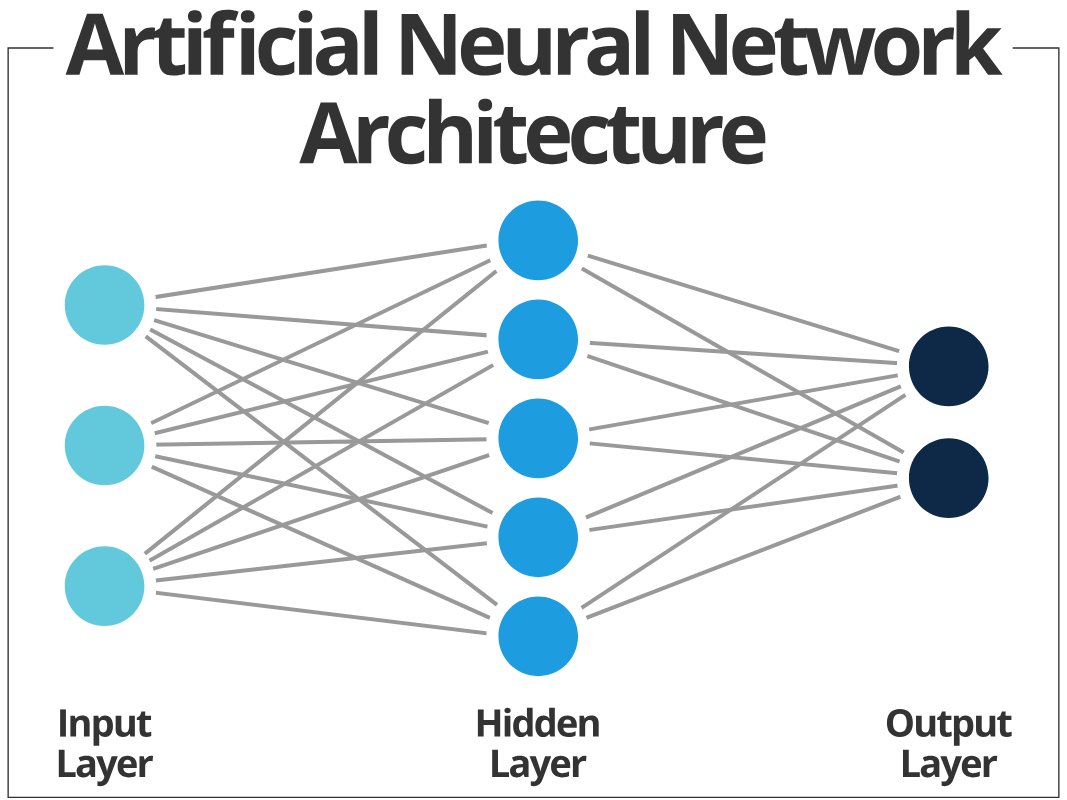
\includegraphics[width=0.7\textwidth,keepaspectratio=true]{ANN.png}
    \caption{Simplified view of the architecture of an Artificial Neural Network ~\cite{Image:ANN}}
\end{figure}
\clearpage
\subsection{Appendix B: K-12 AI Curricula}\label{app:b}
\begin{table}[htpb]
\centering
\resizebox{\linewidth}{!}{%
\begin{tabular}{llllll}
\hline
\textbf{} & \textbf{Curriculum title} & \textbf{Curriculum developer} & \textbf{Educational levels} & \textbf{} & \textbf{} \\ \hline
\textbf{} & ~ & ~ & Primary & Middle & High \\ 
\textbf{Armenia} & Curriculum of ICT & Government & ~ & X & X \\ 
\textbf{Austria} & Data Science and Artificial Intelligence & Federal Ministry of Education, Science and & ~ & ~ & X \\ 
\textbf{} & ~ & Research & ~ & ~ & ~ \\ 
\textbf{Belgium} & IT Repository & Fédération Wallonie-Bruxelles (French-speaking & ~ & ~ & X \\ 
\textbf{} & ~ & Community of Belgium) & ~ & ~ & ~ \\ 
\textbf{China} & AI curriculum embedded in the & The Ministry of Education of the People’s & X & X & X \\ 
\textbf{} & Information Science and Technology & Republic of China & ~ & ~ & ~ \\ 
\textbf{} & curriculum & ~ & ~ & ~ & ~ \\ 
\textbf{India} & Atal Tinker Labs AI modules & Atal Tinker Labs, Atal Innovation Mission, NITI & ~ & X & X \\ 
\textbf{} & ~ & Aayoag & ~ & ~ & ~ \\ 
\textbf{Republic of Korea} & ‘AI Mathematics’ under the Mathematics & Korea Foundation for the Advancement of & ~ & ~ & X \\ 
\textbf{} & Subject Group for high schools & Science and Creativity & ~ & ~ & ~ \\ 
\textbf{} & ‘AI Basics’ under Technology Home & Korea Foundation for the Advancement of & ~ & ~ & X \\ 
\textbf{} & Economics Subject Group for high & Science and Creativity & ~ & ~ & ~ \\ 
\textbf{} & schools & ~ & ~ & ~ & ~ \\ 
\textbf{Kuwait} & Standards curriculum & Curricula technical guidance experts and & X & X & ~ \\ 
\textbf{} & ~ & teachers & ~ & ~ & ~ \\ 
\textbf{Portugal} & Information and Communication & State school teachers of ICT and Mathematics & X & X & X \\ 
\textbf{} & Technologies & ~ & ~ & ~ & ~ \\ 
\textbf{Qatar} & Computing and Information Technology & Binary Logic, Ministry of Education and Higher & X & X & X \\ 
\textbf{} & ~ & Education & ~ & ~ & ~ \\ 
\textbf{} & Computing and Information Technology & Binary Logic, Ministry of Education and Higher & ~ & ~ & X \\ 
\textbf{} & (High Tech Track) & Education & ~ & ~ & ~ \\ 
\textbf{Serbia} & Informatics and programming – Grade 8 & Ministry of Education working group & ~ & X & ~ \\ 
\textbf{} & Modern technologies in gymnasiums – Grade 3 and 4 & Ministry of Education working group & ~ & ~ & X \\ 
\textbf{United Arab Emirates} & AI curriculum embedded under the
Technology Subject Framework & Ministry of Education & X & X & X \\\hline
\hline
\end{tabular}%
}
\caption{K-12 AI Curricula, endorsed and implemented by governments vs. country/region ~\cite{worldwide-adoption}}
\end{table}
\clearpage
\subsection{Appendix C: Simplified View Strategies}\label{app:c}
\begin{figure}[htpb]
    \centering
    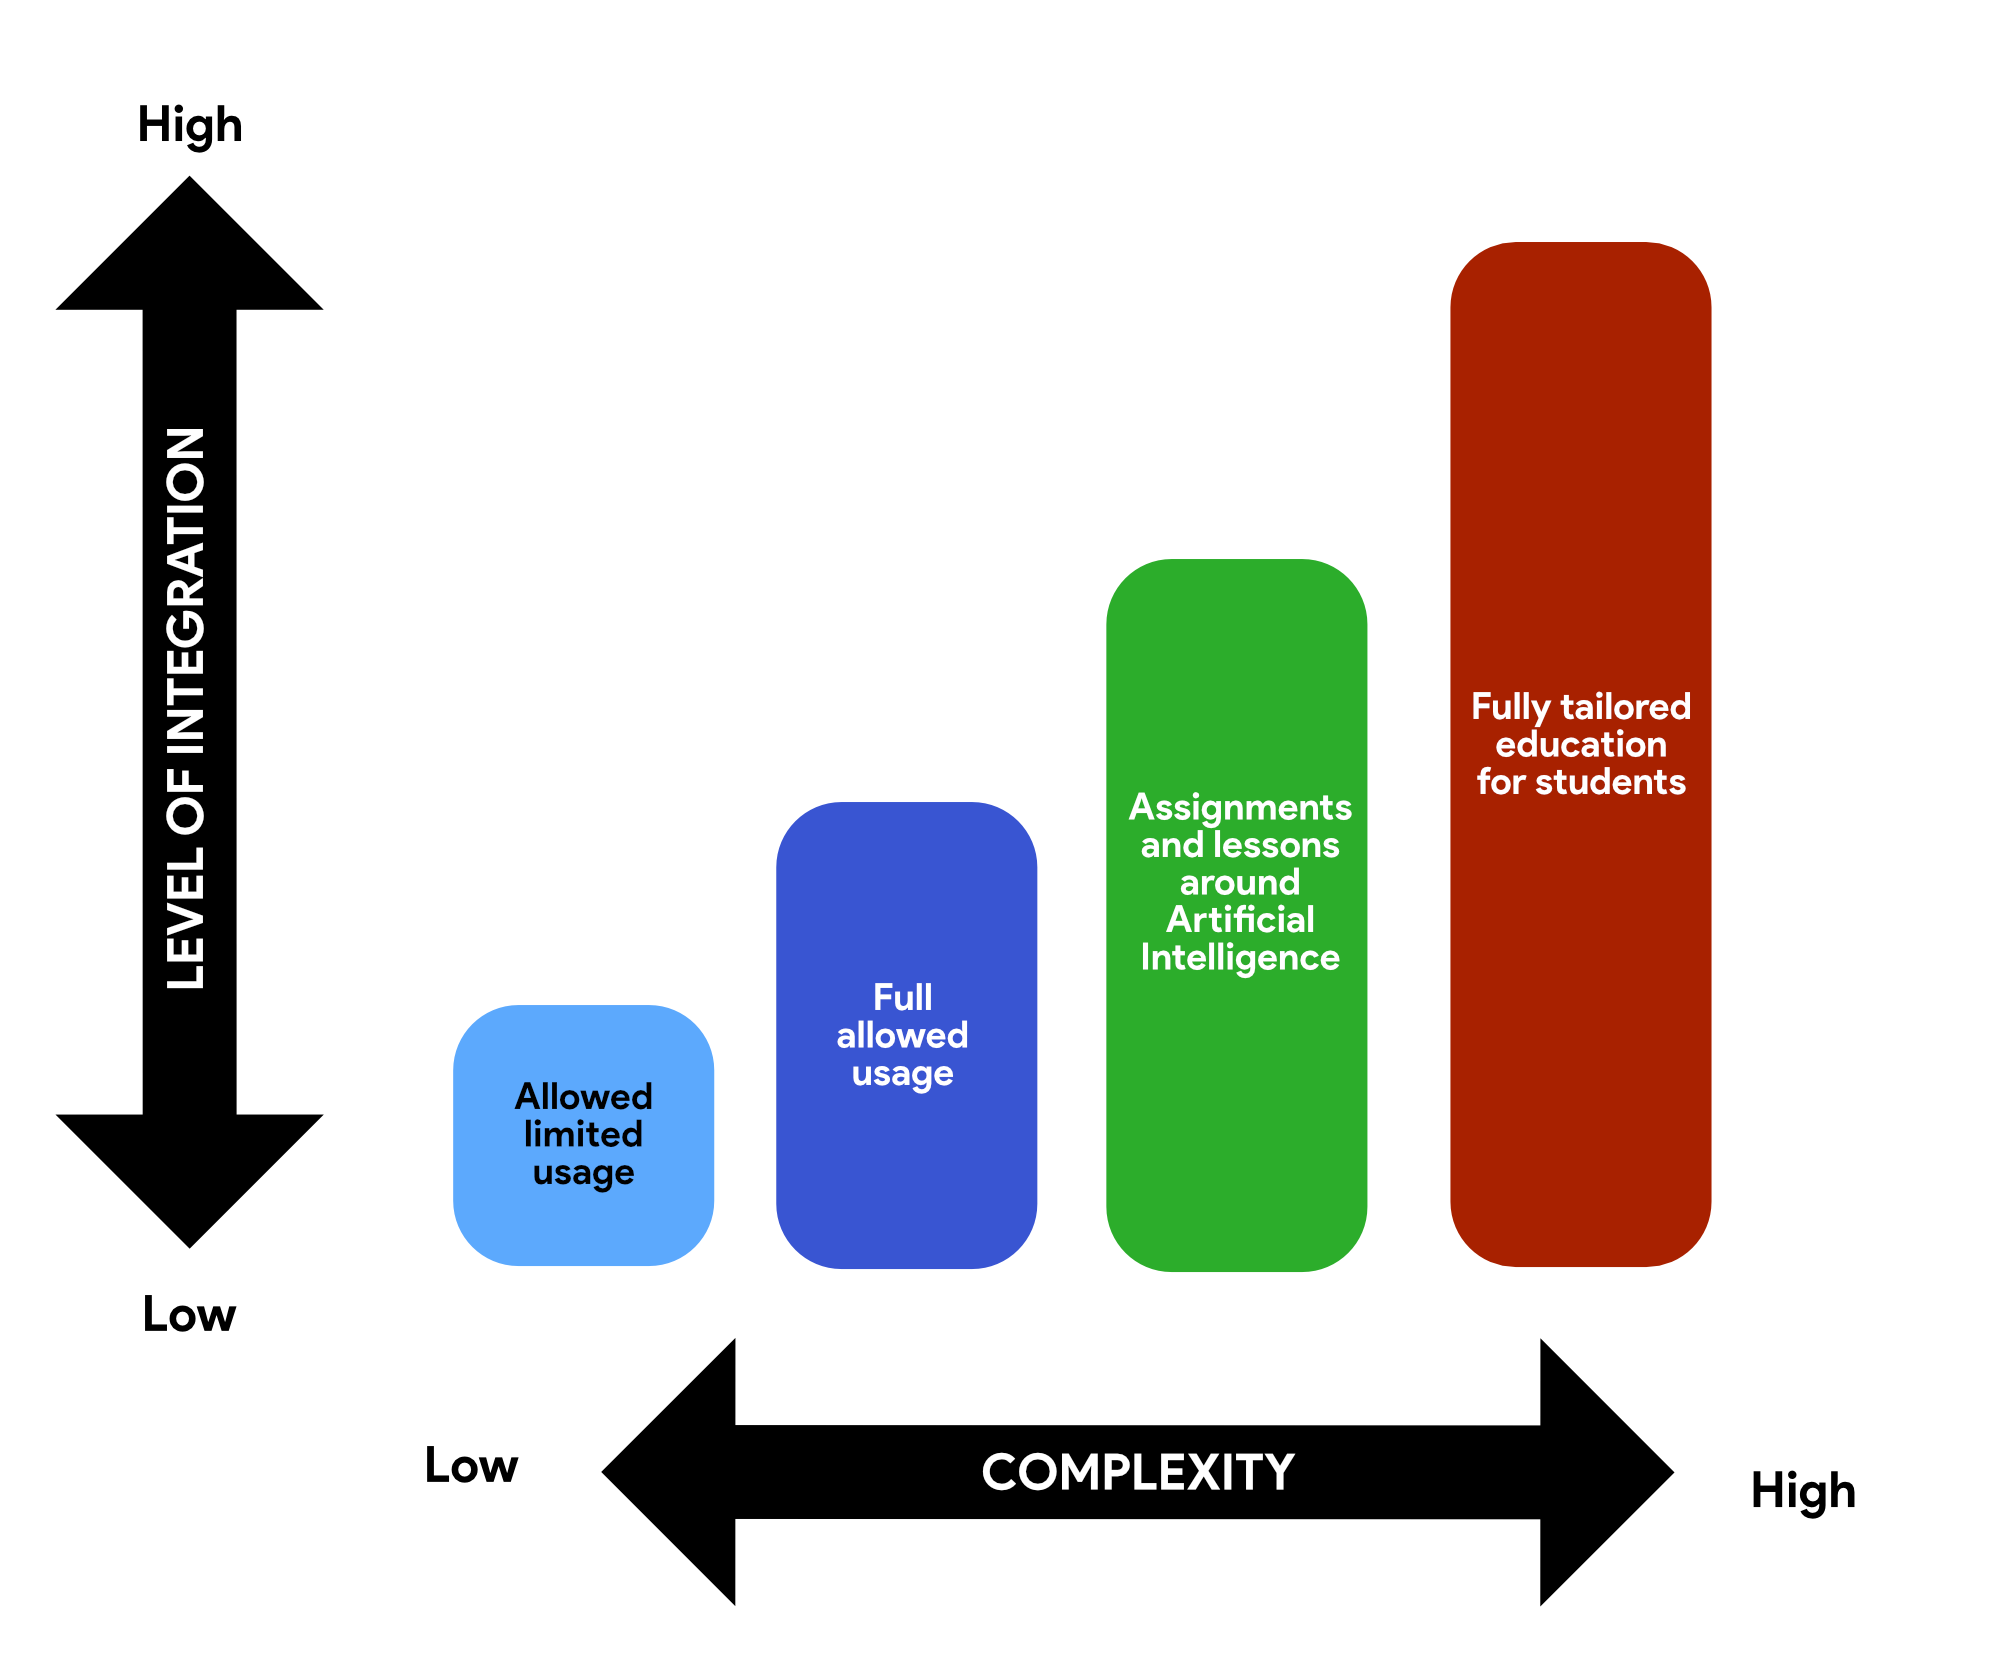
\includegraphics[width=0.7\textwidth,keepaspectratio=true]{Graph 1 PWS.png}
    \caption{Simplified view of the strategies for integrating Artificial Intelligence from the optic of pupils}
\end{figure}

\newpage
\begingroup
\section{Bibliography} \label{sect:bibliography}
\let\clearpage\relax
\renewcommand{\bibname}{}
\bibliographystyle{apalike}
\bibliography{bibliography}
\endgroup

\newpage
\section*{Bijlagen} \label{sect:bijlagen}
\thispagestyle{empty}
\subsection*{Logboek}
\hspace*{-3.5cm}
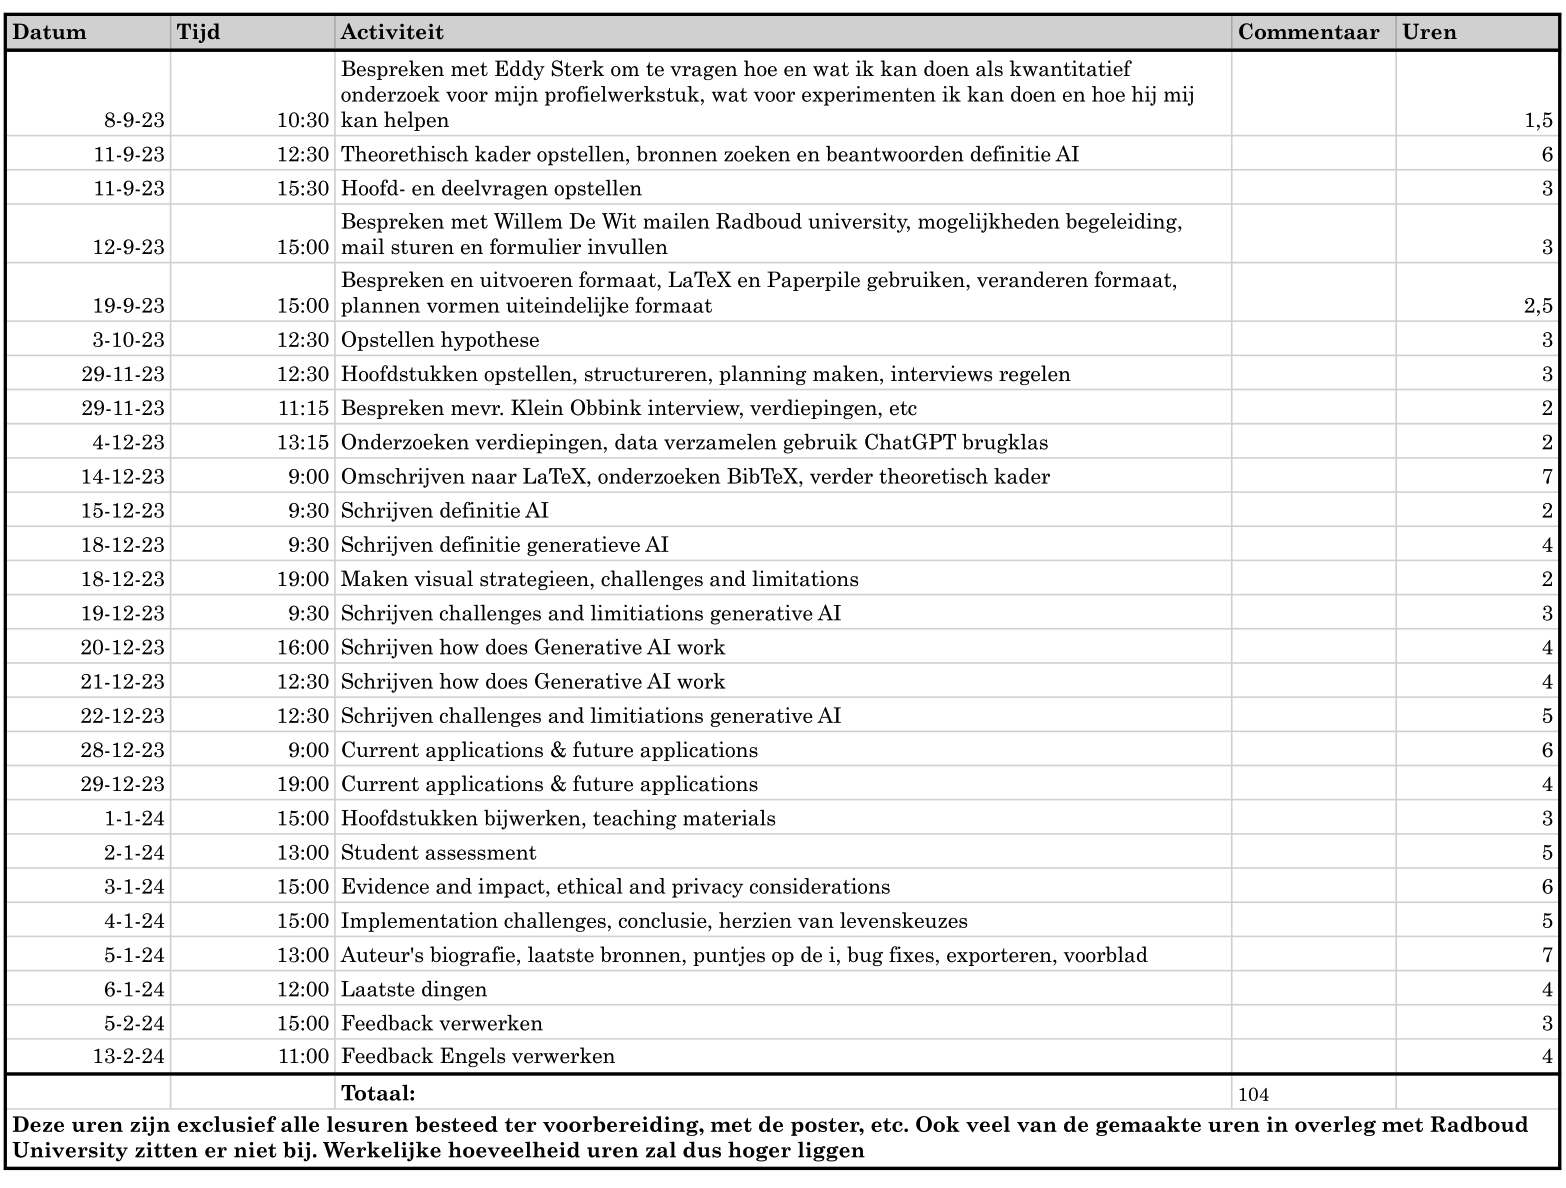
\includegraphics[width=1.385\textwidth,keepaspectratio=true]{Logboek.png}
\end{document}